\section{Download and install}\label{sec:dai}
%
You will need Virtual Box, because some components of the SailfishOS SDK come as virtual machines. Download for your development machine\cite{vbox01}.
%
\begin{figure}[H]
  \centering
  \includegraphics[scale=0.4]{../media/gfx/VirtualBox/vboxdownload.png} 
  \caption{Download VirtualBox from the virtualbox website.}
  \label{fig:vboxdownload}
\end{figure}
%
If you already use VirtualBox, you don't need to load it again, just skip that step. Just make sure that you have the latest updates installed.

To take a dip, head over to the Sailfish Website\cite{sailfishos01} and download the SDK for your operating system.
%
\begin{figure}[H]
  \centering
  \includegraphics[scale=0.4]{../media/gfx/Sailfish/downloadsdk.png} 
  \caption{Download the SDK from the SailfishOS website.}
  \label{fig:downloadsdk}
\end{figure}
%
\subsection{OSX}\label{subsec:osxinstall}
%
Double click on the downloaded disk image for VirtualBox and run the installer application inside. Some file go into system folders and you must be or elevate to an admin account to install successfully.
\begin{figure}[H]
  \centering
  \includegraphics[scale=0.2]{../media/gfx/OSX/osxdiskimage.png} 
  \caption{Downloaded diskimage.}
  \label{fig:osxdiskimage}
\end{figure}
%
%
\begin{figure}[H]
  \centering
  \includegraphics[scale=0.5]{../media/gfx/VirtualBox/vboxosxinstall01.png} 
  \caption{Install VirtualBox, step 1.}
  \label{fig:vboxosxinstall01}
\end{figure}
%
%
\begin{figure}[H]
  \centering
  \includegraphics[scale=0.5]{../media/gfx/VirtualBox/vboxosxinstall02.png} 
  \caption{Install VirtualBox, step 2.}
  \label{fig:vboxosxinstall02}
\end{figure}
%
%
\begin{figure}[H]
  \centering
  \includegraphics[scale=0.5]{../media/gfx/VirtualBox/vboxosxinstall03.png} 
  \caption{Install VirtualBox, step 3.}
  \label{fig:vboxosxinstall03}
\end{figure}
%
%
\begin{figure}[H]
  \centering
  \includegraphics[scale=0.5]{../media/gfx/VirtualBox/vboxosxinstall04.png} 
  \caption{Install VirtualBox, step 4.}
  \label{fig:vboxosxinstall04}
\end{figure}
%
%
\begin{figure}[H]
  \centering
  \includegraphics[scale=0.5]{../media/gfx/VirtualBox/vboxosxinstall05.png} 
  \caption{Install VirtualBox, step 5.}
  \label{fig:vboxosxinstall05}
\end{figure}
%
If you use VirtualBox just for the SailfishOS SDK you don't have to care about the VirtualBox application, although you can see which folders are shared inside the preferences.

Double click on the downloaded disk image for the SailfishOS SDK and run the installer app that's inside. The installed files will end in your user directory, you don't need to be an administrator to achieve that.
%
\begin{figure}[H]
  \centering
  \includegraphics[scale=0.6]{../media/gfx/OSX/installsdk01.png} 
  \caption{Install SailfishOS SDK, step 1.}
  \label{fig:installsdk01}
\end{figure}
%
%
\begin{figure}[H]
  \centering
  \includegraphics[scale=0.6]{../media/gfx/OSX/installsdk02.png} 
  \caption{Install SailfishOS SDK, step 2.}
  \label{fig:installsdk02}
\end{figure}
%
Since the Alpha2 SDK you can select a separate folder for your source code if it is stored outside your home folder. Since the Alpha3 SDK this setting should work.
%
\begin{figure}[H]
  \centering
  \includegraphics[scale=0.6]{../media/gfx/OSX/installsdk03.png} 
  \caption{Install SailfishOS SDK, step 3. Enter the path to your source code. There is no folder selector dialog, you must enter it by hand.}
  \label{fig:installsdk03}
\end{figure}
%
%
\begin{figure}[H]
  \centering
  \includegraphics[scale=0.6]{../media/gfx/OSX/installsdk04.png} 
  \caption{Install SailfishOS SDK, step 4.}
  \label{fig:installsdk04}
\end{figure}
%
The Alpha3 SDK added a screen here, where you (de-)select components.
%
\begin{figure}[H]
  \centering
  \includegraphics[scale=0.6]{../media/gfx/OSX/installsdk05.png} 
  \caption{Install SailfishOS SDK, step 5.}
  \label{fig:installsdk05}
\end{figure}
%
%
\begin{figure}[H]
  \centering
  \includegraphics[scale=0.6]{../media/gfx/OSX/installsdk06.png} 
  \caption{Install SailfishOS SDK, step 6.}
  \label{fig:installsdk06}
\end{figure}
%
%
\begin{figure}[H]
  \centering
  \includegraphics[scale=0.6]{../media/gfx/OSX/installsdk07.png} 
  \caption{Install SailfishOS SDK, step 7.}
  \label{fig:installsdk07}
\end{figure}
%
%
\begin{figure}[H]
  \centering
  \includegraphics[scale=0.6]{../media/gfx/OSX/installsdk08.png} 
  \caption{Unmount SailfishOS SDK disk image, step 8.}
  \label{fig:installsdk08}
\end{figure}
%
With the installation came two hidden directories, you should know about. More about those directories will follow later on.
\\
\\
\verb,$HOME/.config/SailfishAlpha3,\\
\verb,$HOME/.scratchbox2,\\
\\
After you installed the SDK, you should immediately update the components.
%
\begin{figure}[H]
  \centering
  \includegraphics[scale=0.6]{../media/gfx/QtCreator/QtCreatorUpdateNeeded.png} 
  \caption{QtCreator show that there are updates for the SDK.}
  \label{fig:QtCreatorUpdateNeeded}
\end{figure}
%
As of now the progress inside Jolla is at good pace, so it might be that there is some stuff slightly out of date in the installer (see figures \ref{fig:osxupdate} and \ref{fig:osxupdate2}).
%
\begin{figure}[H]
  \centering
  \includegraphics[scale=0.8]{../media/gfx/OSX/OSXSDKMaintenaceTool.png} 
  \caption{Inside the SailfishOS folder you find the maintenance application. Run it directly after the installation.}
  \label{fig:osxupdate}
\end{figure}
%
%
\begin{figure}[H]
  \centering
  \includegraphics[scale=0.6]{../media/gfx/OSX/OSXSDKMaintenaceTool_run.png} 
  \caption{Update components, choose everything that is in store.}
  \label{fig:osxupdate2}
\end{figure}
%
With the SDK comes QtCreator\footnote{Look in in the "bin" folder of the SDK.}, a complete IDE for C++ development. This IDE is part of the Qt Framework\cite{qt01} and is simply reused\footnote{Customized with some little tweaks to suite the SailfishOS development.}by Jolla. Personally I use the QtCreator on my machines as well and for better differentiation I made a custom icon for the one in the SailfishOS SDK - feel free to download and use it, too\cite{hc03}.
\begin{figure}[H]
  \centering
  \includegraphics[scale=3.0]{../media/gfx/Sailfish/Sailfish_Logo_Ocean.png} 
  \caption{Alternative icon for the QtCreator inside the SDK.}
  \label{fig:sdklogocustom}
\end{figure}
%
%
\subsection{Windows}
%
Double click the $\vcenter{\hbox{\includegraphics[scale=0.6]{../media/gfx/VirtualBox/vboxinstaller.png}}}$ executable that you have downloaded and follow the installer.
%
\begin{figure}[H]
  \centering
  \includegraphics[scale=0.6]{../media/gfx/VirtualBox/vboxinstwin01.png} 
  \caption{Install VirtualBox, Step 1.}
  \label{fig:vboxinstwin01}
\end{figure}
%
%
\begin{figure}[H]
  \centering
  \includegraphics[scale=0.6]{../media/gfx/VirtualBox/vboxinstwin02.png} 
  \caption{Install VirtualBox, Step 2.}
  \label{fig:vboxinstwin02}
\end{figure}
%
%
\begin{figure}[H]
  \centering
  \includegraphics[scale=0.6]{../media/gfx/VirtualBox/vboxinstwin03.png} 
  \caption{Install VirtualBox, Step 3.}
  \label{fig:vboxinstwin03}
\end{figure}
%
\begin{figure}[H]
  \centering
  \includegraphics[scale=0.6]{../media/gfx/VirtualBox/vboxinstwin04.png} 
  \caption{Install VirtualBox, Step 4.}
  \label{fig:vboxinstwin01}
\end{figure}
%
\begin{figure}[H]
  \centering
  \includegraphics[scale=0.6]{../media/gfx/VirtualBox/vboxinstwin05.png} 
  \caption{Install VirtualBox, Step 5.}
  \label{fig:vboxinstwin05}
\end{figure}
%
\begin{figure}[H]
  \centering
  \includegraphics[scale=0.6]{../media/gfx/VirtualBox/vboxinstwin06.png} 
  \caption{Install VirtualBox, Step 6.}
  \label{fig:vboxinstwin06}
\end{figure}
%
\begin{figure}[H]
  \centering
  \includegraphics[scale=0.6]{../media/gfx/VirtualBox/vboxinstwin07.png} 
  \caption{Install VirtualBox, Step 7.}
  \label{fig:vboxinstwin07}
\end{figure}
%
\begin{figure}[H]
  \centering
  \includegraphics[scale=0.6]{../media/gfx/VirtualBox/vboxinstwin08.png} 
  \caption{Install VirtualBox, Step 8.}
  \label{fig:vboxinstwin08}
\end{figure}
%
\begin{figure}[H]
  \centering
  \includegraphics[scale=0.6]{../media/gfx/VirtualBox/vboxinstwin09.png} 
  \caption{Install VirtualBox, Step 9.}
  \label{fig:vboxinstwin09}
\end{figure}
%
\begin{figure}[H]
  \centering
  \includegraphics[scale=0.6]{../media/gfx/VirtualBox/vboxinstwin10.png} 
  \caption{Install VirtualBox, Step 10.}
  \label{fig:vboxinstwin10}
\end{figure}
%
\begin{figure}[H]
  \centering
  \includegraphics[scale=0.6]{../media/gfx/VirtualBox/vboxinstwin11.png} 
  \caption{Install VirtualBox, Step 11.}
  \label{fig:vboxinstwin11}
\end{figure}
%
Start the $\vcenter{\hbox{
\includegraphics[scale=0.6]{../media/gfx/Windows/sfosinstaller.png}}}$ executable and install the SDK.
%
\begin{figure}[H]
  \centering
  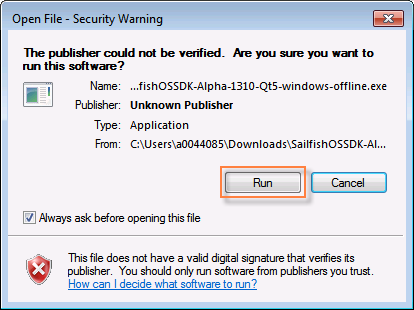
\includegraphics[scale=0.6]{../media/gfx/Windows/installsdkwin01.png} 
  \caption{Install SDK, Step 1.}
  \label{fig:installsdkwin01}
\end{figure}
%
\begin{figure}[H]
  \centering
  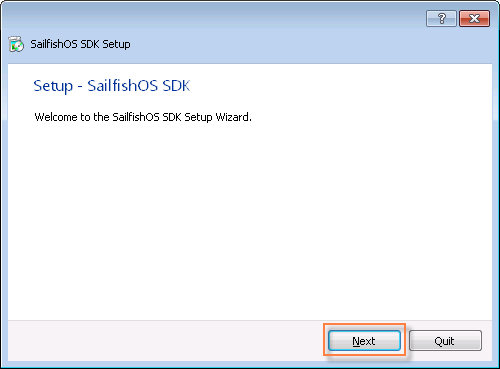
\includegraphics[scale=0.6]{../media/gfx/Windows/installsdkwin02.png} 
  \caption{Install SDK, Step 2.}
  \label{fig:installsdkwin02}
\end{figure}
%
\begin{figure}[H]
  \centering
  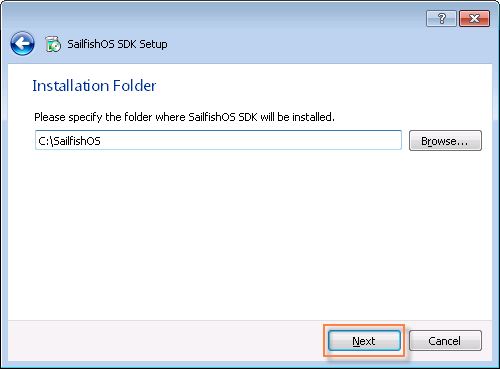
\includegraphics[scale=0.6]{../media/gfx/Windows/installsdkwin03.png} 
  \caption{Install SDK, Step 3.}
  \label{fig:installsdkwin03}
\end{figure}
%
\begin{figure}[H]
  \centering
  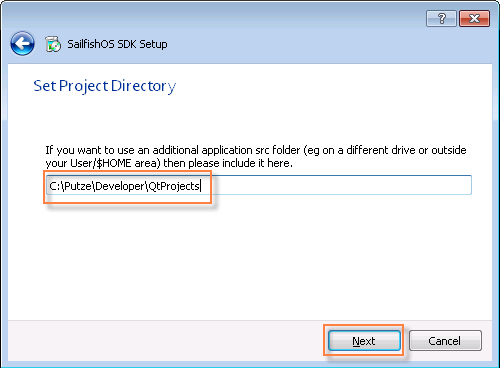
\includegraphics[scale=0.6]{../media/gfx/Windows/installsdkwin04.png} 
  \caption{Install SDK, Step 4.}
  \label{fig:installsdkwin04}
\end{figure}
%
\begin{figure}[H]
  \centering
  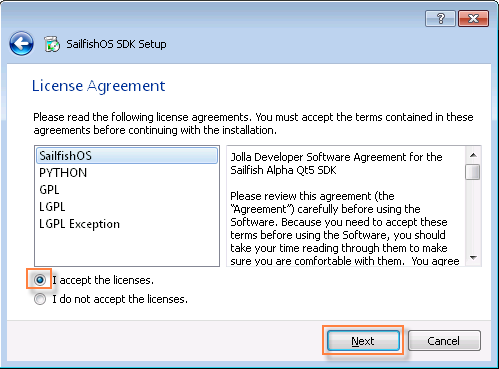
\includegraphics[scale=0.6]{../media/gfx/Windows/installsdkwin05.png} 
  \caption{Install SDK, Step 5.}
  \label{fig:installsdkwin05}
\end{figure}
%
\begin{figure}[H]
  \centering
  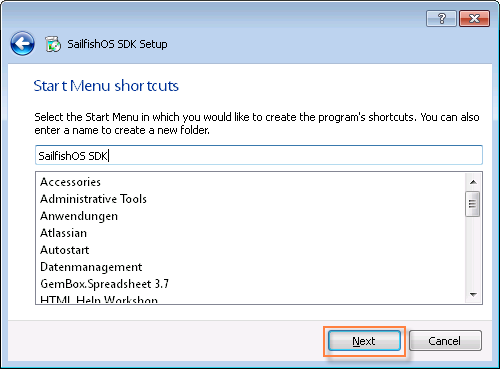
\includegraphics[scale=0.6]{../media/gfx/Windows/installsdkwin06.png} 
  \caption{Install VirtualBox, Step 6.}
  \label{fig:installsdkwin06}
\end{figure}
%
\begin{figure}[H]
  \centering
  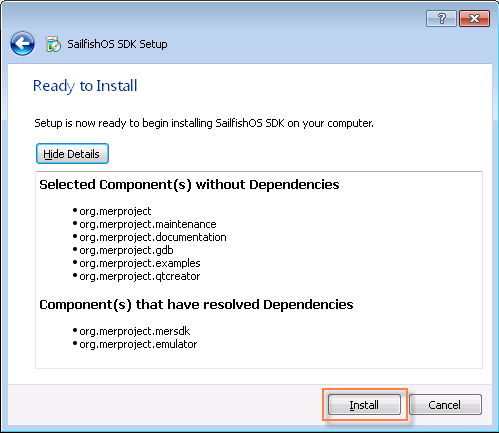
\includegraphics[scale=0.6]{../media/gfx/Windows/installsdkwin07.png} 
  \caption{Install VirtualBox, Step 7.}
  \label{fig:installsdkwin07}
\end{figure}
%
\begin{figure}[H]
  \centering
  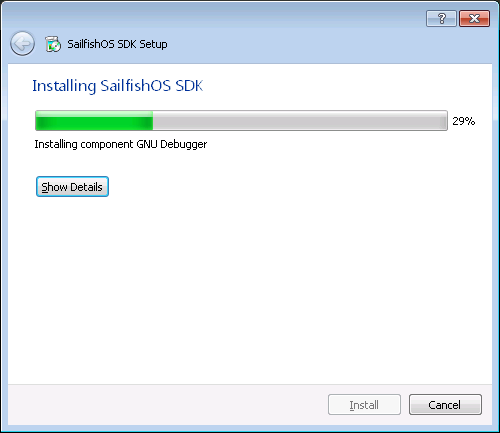
\includegraphics[scale=0.6]{../media/gfx/Windows/installsdkwin08.png} 
  \caption{Install VirtualBox, Step 8.}
  \label{fig:installsdkwin08}
\end{figure}
%
\begin{figure}[H]
  \centering
  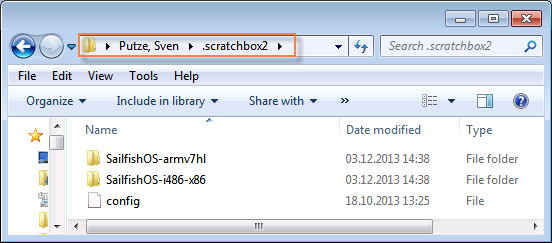
\includegraphics[scale=0.6]{../media/gfx/Windows/installsdkwin09.png} 
  \caption{Install VirtualBox, Step 9.}
  \label{fig:installsdkwin09}
\end{figure}
%
Start the maintenance tool from the start menu or from the SailfishOS SDK directory $\vcenter{\hbox{
\includegraphics[scale=0.8]{../media/gfx/Windows/sdkmaintenacetoolwin.png}}}$ and update all components.
%
\begin{figure}[H]
  \centering
  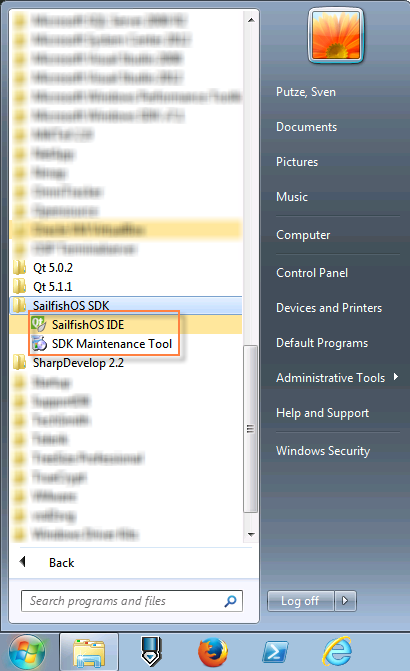
\includegraphics[scale=0.6]{../media/gfx/Windows/sdkwinstartmenu.png} 
  \caption{SDK and maintenance tool}
  \label{fig:sdkwinstartmenu}
\end{figure}
%
With the installation come some directories.
%
\begin{figure}[H]
  \centering
  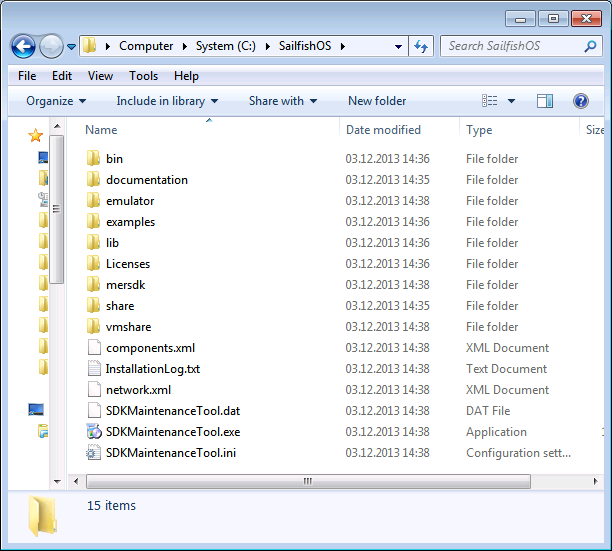
\includegraphics[scale=0.6]{../media/gfx/Windows/sdkdirwin01.png} 
  \caption{Directory after installation.}
  \label{fig:saddirwin01}
\end{figure}
%
%
\begin{figure}[H]
  \centering
  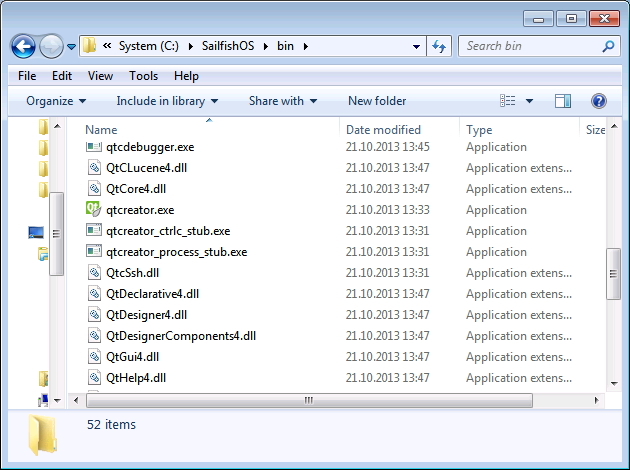
\includegraphics[scale=0.6]{../media/gfx/Windows/sdkdirwin02.png} 
  \caption{Directory after installation.}
  \label{fig:saddirwin02}
\end{figure}
%
%
%
\subsection{Linux}
%
Download the Linux installer from the VirtualBox homepage. My distribution of choice is Debian based, so I chose the 64bit Debian package. Open your terminal and install with
%
\begin{figure}[H]
  \centering
  \includegraphics[scale=0.4]{../media/gfx/VirtualBox/vboxlinux01-01.png} 
  \caption{Install VirtualBox from the terminal.}
  \label{fig:vboxlinux01-01}
\end{figure}
%
\begin{lstlisting}[language=bash]
cd downloads
sudo dpkg --install ./virtualbox-4.3_4.3.4-91027~Debian~wheezy_amd64.deb
# as you can see in the screenshot there are missing dependencies, install them with
sudo apt-get -f install
# and now finish the installation
sudo dpkg --install ./virtualbox-4.3_4.3.4-91027~Debian~wheezy_amd64.deb
\end{lstlisting}
%
Now download the installer from \cite{sailfishos01},
%
\begin{figure}[H]
  \centering
  \includegraphics[scale=0.6]{../media/gfx/Linux/linux01-01.png} 
  \caption{Install SailfishOS SDK on Linux, step 1.}
  \label{fig:vboxlinux01-01}
\end{figure}
%
make it executable and start it. From now on it's mostly like on OSX and/or Windows.
%
\begin{figure}[H]
  \centering
  \includegraphics[scale=0.4]{../media/gfx/Linux/linux01-02.png} 
  \caption{Install SailfishOS SDK on Linux, step 2.}
  \label{fig:vboxlinux01-02}
\end{figure}
%
%
\begin{figure}[H]
  \centering
  \includegraphics[scale=0.6]{../media/gfx/Linux/linux01-04.png} 
  \caption{Install SailfishOS SDK on Linux, step 4.}
  \label{fig:vboxlinux01-04}
\end{figure}
%
%
\begin{figure}[H]
  \centering
  \includegraphics[scale=0.6]{../media/gfx/Linux/linux01-05.png} 
  \caption{Install SailfishOS SDK on Linux, step 5.}
  \label{fig:vboxlinux01-05}
\end{figure}
%
%
\begin{figure}[H]
  \centering
  \includegraphics[scale=0.6]{../media/gfx/Linux/linux01-06.png} 
  \caption{Install SailfishOS SDK on Linux, step 6.}
  \label{fig:vboxlinux01-06}
\end{figure}
%
%
\begin{figure}[H]
  \centering
  \includegraphics[scale=0.6]{../media/gfx/Linux/linux01-07.png} 
  \caption{Install SailfishOS SDK on Linux, step 7.}
  \label{fig:vboxlinux01-07}
\end{figure}
%
%
\begin{figure}[H]
  \centering
  \includegraphics[scale=0.6]{../media/gfx/Linux/linux01-08.png} 
  \caption{Install SailfishOS SDK on Linux, step 8.}
  \label{fig:vboxlinux01-08}
\end{figure}
%
%
\begin{figure}[H]
  \centering
  \includegraphics[scale=0.6]{../media/gfx/Linux/linux01-09.png} 
  \caption{Install SailfishOS SDK on Linux, step 9.}
  \label{fig:vboxlinux01-09}
\end{figure}
%
Now you can start and use the SDK. How to start depends on your distribution. Maybe a menu entry was created, maybe you must create one on your own. The binary is in the \verb,~/SailfishOS/bin, folder\footnote{If you have chosen the default location, of course.}.
%
%
\subsection{Remove plugins}\label{subsec:removeplugins}
%
If you want to improve the startup time of QtCreator, you can deactivate plugins you don't need or want\footnote{On Windows and Linux the plugins should be found in Extras/Plugins.}. Just don't shoot in your foot here.
%
\begin{figure}[H]
  \centering
  \includegraphics[scale=0.6]{../media/gfx/QtCreator/qtcreatorplugins.png} 
  \caption{About plugins = manage plugins.}
  \label{fig:qtcreatorplugins}
\end{figure}
%
\begin{figure}[H]
  \centering
  \includegraphics[scale=0.6]{../media/gfx/QtCreator/qtcreatordeactivateplugin.png} 
  \caption{Deactivate every plugin you don't need.}
  \label{fig:qtcreatordeactivateplugin}
\end{figure}
%
